\documentclass[tikz,border=10pt]{standalone}
\usetikzlibrary{angles}
\begin{document}
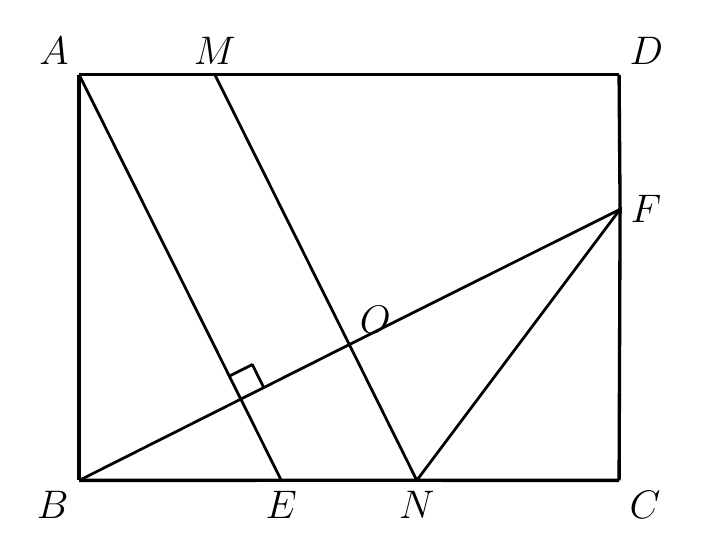
\begin{tikzpicture}[line width=1.0pt, line join=round]
\coordinate (A) at (-3.456,2.585);
\coordinate (B) at (-3.456,-2.567);
\coordinate (C) at (3.401,-2.567);
\coordinate (D) at (3.401,2.585);
\coordinate (F) at (3.414,0.876);
\coordinate (M) at (-1.732,2.585);
\coordinate (N) at (0.832,-2.566);
\coordinate (O) at (-0.025,-0.842);




\coordinate (E) at (-0.889,-2.566);
\coordinate (P) at (-1.403,-1.535);


\draw[line width=1.2pt] (A) -- (M) -- (D);          
\draw[line width=1.2pt] (B) -- (E) -- (N) -- (C);   
\draw[line width=1.2pt] (D) -- (F) -- (C);          
\draw[line width=1.2pt] (A) -- (B);                 


\draw (A) -- (E);
\draw (B) -- (O) -- (F);
\draw (M) -- (O) -- (N);
\draw (F) -- (N);


\draw pic[draw, angle radius=0.327cm] {right angle=F--P--A};


\node[above left]  at (A) {\fontsize{14.5}{17.4}\selectfont $A$};
\node[above]       at (M) {\fontsize{14.5}{17.4}\selectfont $M$};
\node[above right] at (D) {\fontsize{14.5}{17.4}\selectfont $D$};
\node[right]       at (F) {\fontsize{14.5}{17.4}\selectfont $F$};
\node[above right] at (O) {\fontsize{14.5}{17.4}\selectfont $O$};
\node[below right] at (C) {\fontsize{14.5}{17.4}\selectfont $C$};
\node[below left]  at (B) {\fontsize{14.5}{17.4}\selectfont $B$};
\node[below]       at (E) {\fontsize{14.5}{17.4}\selectfont $E$};
\node[below]       at (N) {\fontsize{14.5}{17.4}\selectfont $N$};
\end{tikzpicture}
\end{document}